TODO amdhal \'e un casino quindi tanto vale mettere lo schedule nel cap 3


TODO servirebbero le misure fatte usando un solo core

TODO
In this chapter I will describe obtained results on each test machine. I will show scheduling executed and improvements on cache miss migration  ...

The scheduling that the developed patch should be perform is showed in fig TODO

TODO dire ideally scheduling
TODO fig schedule

%According to amdhal Law \cite{lcs}:
%	
%\begin{equation}
%       Speedup = (\frac{P_{1}}{S_{1}} + \frac{P_{2}}{S_{2}} + ... \frac{P_{n}}{S_{n}})^{-1} 
%\label{eq:amdhal}
%\end{equation}
%
%We will verify on each tested machine, if developed patch provide the expected speedup.

In this chapter I will show the behaviour of task-affinity on different architectures. First of all, using \textit{trace}, we will check if expected 
scheduling is performed, after which we will analyze how optimization proposed influence performance. We expect a significant improvement of throughput and
predictability that it means a reduction of cache misses.

%%%%%%%%%%%%%%%%%%%%%%%%%%%%%%%%%%%%%%%%%%%%%%%%%%%%%%%%%%%%%%%%%%%%%%%%%%%%%
\section{Intel Xeon}

\begin{figure}[htbp]
\centering
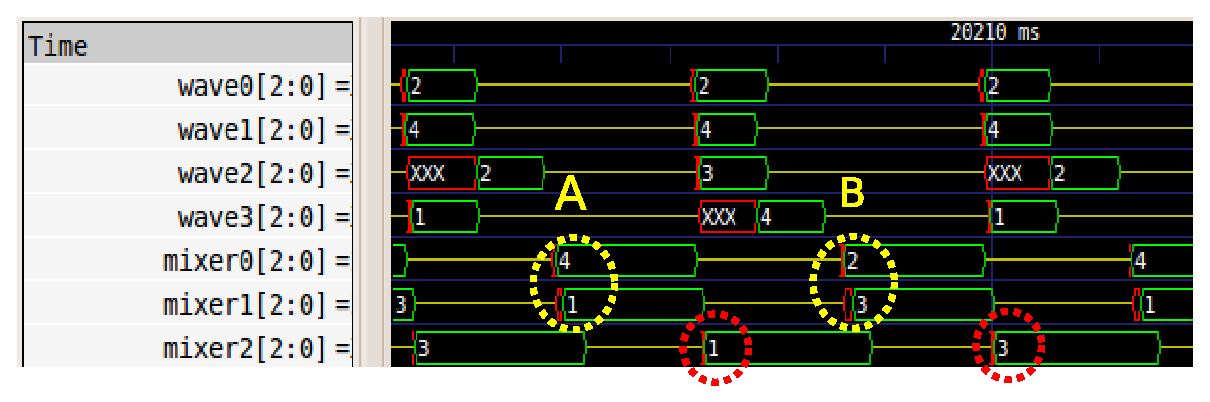
\includegraphics[width=\widefigure]{images/results_xeon/final_xeon.eps}
\caption{\figurecaption{trace TODO dire che sta a 32KB }}
\label{fig:trace_xeon}
\end{figure}

As we can see in Fig. \ref{fig:trace_xeon}, the scheduling performed is correct. We see that \textit{mixer2} can precede one of the waves and improve 
parallelism. We see that \textit{mixer0} chooses the best cpu in term of temporal locality, for example: in step A \textit{mixer0} chooses CPU4 and not 
CPU2, because on CPU2 was executed \textit{wave2}, therefore L1 cache could be dirty, instead on CPU4 the last task executed is \textit{wave1}, therefore 
L1 cache should be clean. Also in step B, it is possible to note how \textit{mixer0} take care about the last task executed on CPU4 choosing CPU2.

\begin{figure}[htbp]
\centering
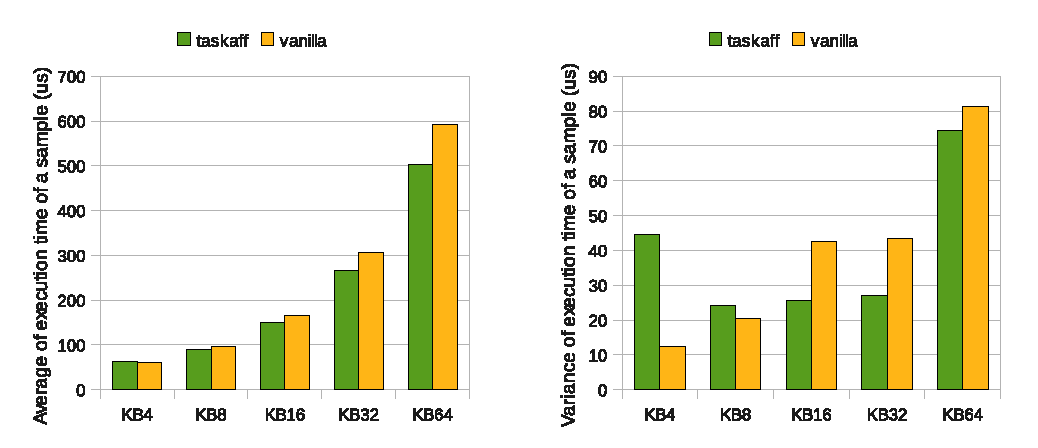
\includegraphics[width=\widefigure]{images/results_xeon/time_avg_var.eps}
\caption{\figurecaption{Average and Variance of execution time of a sample}}
\label{fig:time_avg_var_xeon}
\end{figure}

\begin{figure}[htbp]
\centering
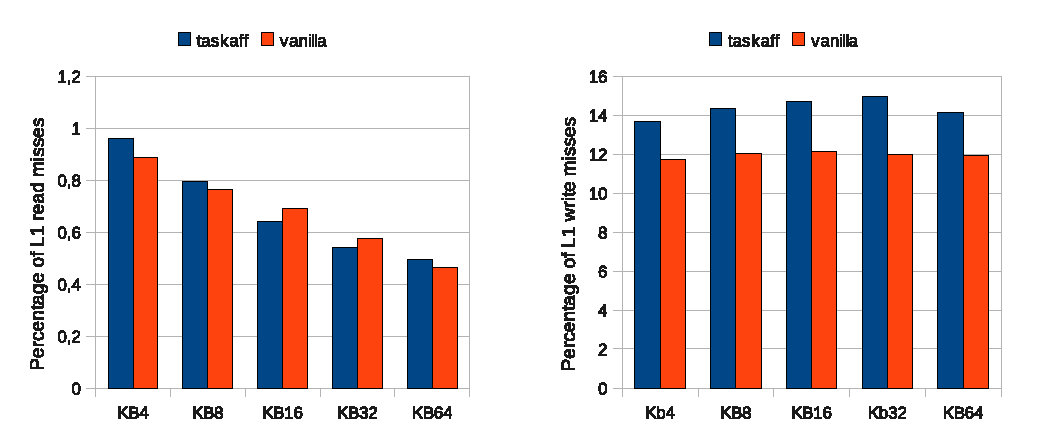
\includegraphics[width=\widefigure]{images/results_xeon/l1_load_store_xeon.eps}
\caption{\figurecaption{L1 Read and Write misses on Xeon}}
\label{fig:l1_load_store_xeon}
\end{figure}

\begin{figure}[htbp]
\centering
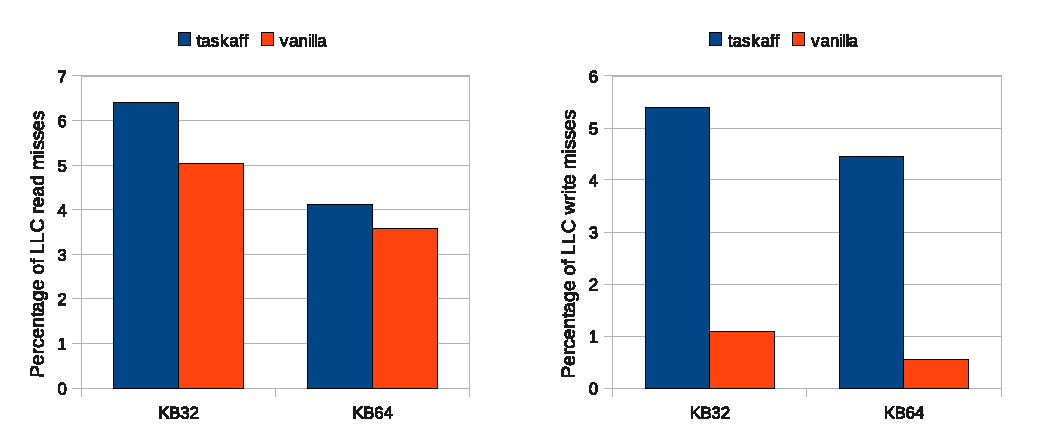
\includegraphics[width=\widefigure]{images/results_xeon/l2_load_store_xeon.eps}
\caption{\figurecaption{LLC Read and Write misses on Xeon}}
\label{fig:l2_load_store_xeon}
\end{figure}

TODO fig. migration

Since parallelism is improved, we can see in Fig \ref{fig:time_avg_var_xeon} an increment of throughput especially with 32 and 64KB, while at 4KB the 
increment is not very significant. This happens because at 4KB tasks are not well parallelized as we can see in Fig. TODO trace 4k

Because of worsening of L1 and LLC cache misses, Fig \ref{fig:l1_load_store_xeon} \ref{fig:l2_load_store_xeon}, predictability of the application is 
degradated, especially using small buffer dimension such as 4KB or 8KB. Nevertheless, with dimension greater than 8KB predictability is improved. Increment 
of cache misses is due to migration, as we can see in Fig. TODO. Number of migration is greatly increased, this fact happens because, at each sample, 
\textit{mixer0} and \textit{mixer1} and waves are excuted on the same CPUs. Since in the next sample waves are waken up during the execution of 
\textit{mixer0} and \textit{mixer1}, they must be scheduled on CPUs different from which that have executed them in the previous sample. For this reason, 
at each sample, waves are executed on different CPUs and, consequently, also other tasks are executed on different CPUs at each sample.

TODO riassumendo tabella speedup

TODO eviterei di metterla
 To explain this fact, it is necessary consider the overhead due to kernel 
functions: \texttt{push\_rt\_task} and \texttt{pull\_rt\_task}


%%%%%%%%%%%%%%%%%%%%%%%%%%%%%%%%%%%%%%%%%%%%%%%%%%%%%%%%%%%%%%%%%%%%%%%%%%%%%
\section{Intel i7}

\begin{figure}[htbp]
\centering
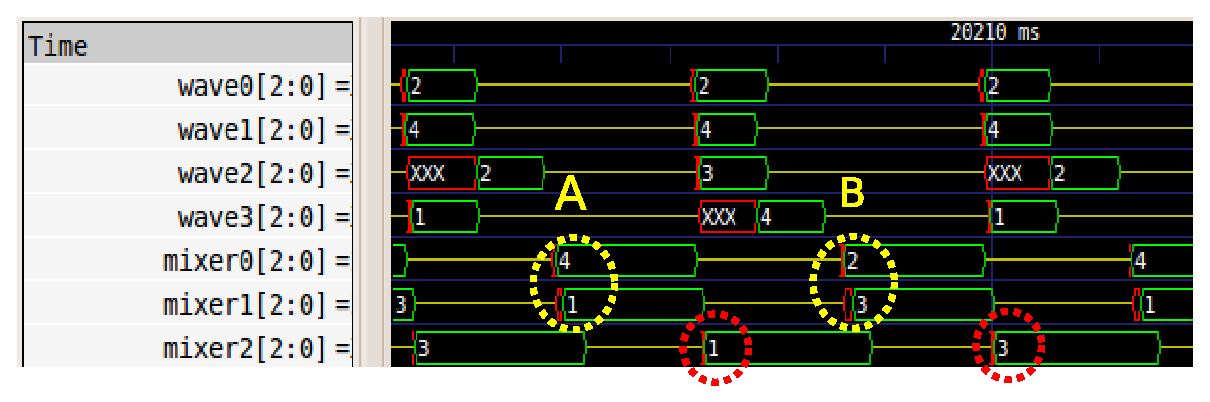
\includegraphics[width=\widefigure]{images/results_xeon/final_xeon.eps}
\caption{\figurecaption{trace TODO}}
\label{fig:trace_i7}
\end{figure}

\begin{figure}[htbp]
\centering
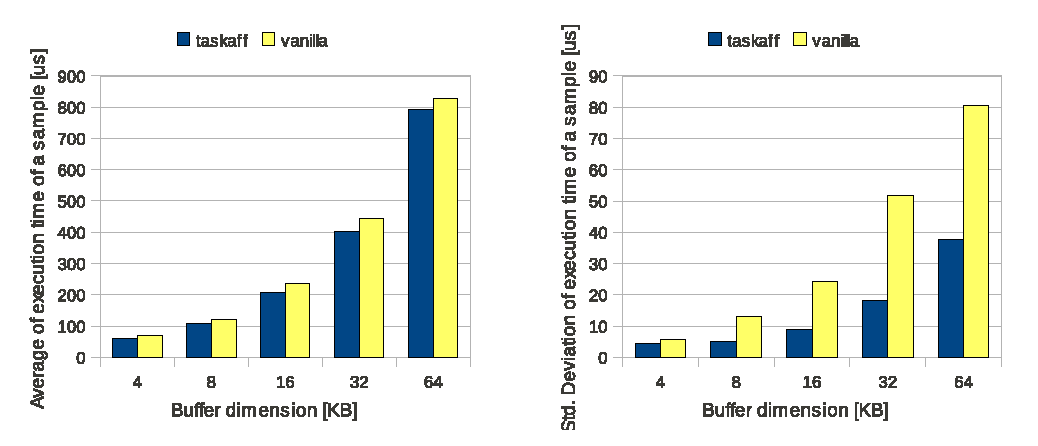
\includegraphics[width=\widefigure]{images/results_i7/time_avg_var_i7.eps}
\caption{\figurecaption{Average and Variance of execution time of a sample}}
\label{fig:time_avg_var_i7}
\end{figure}

\begin{figure}[htbp]
\centering
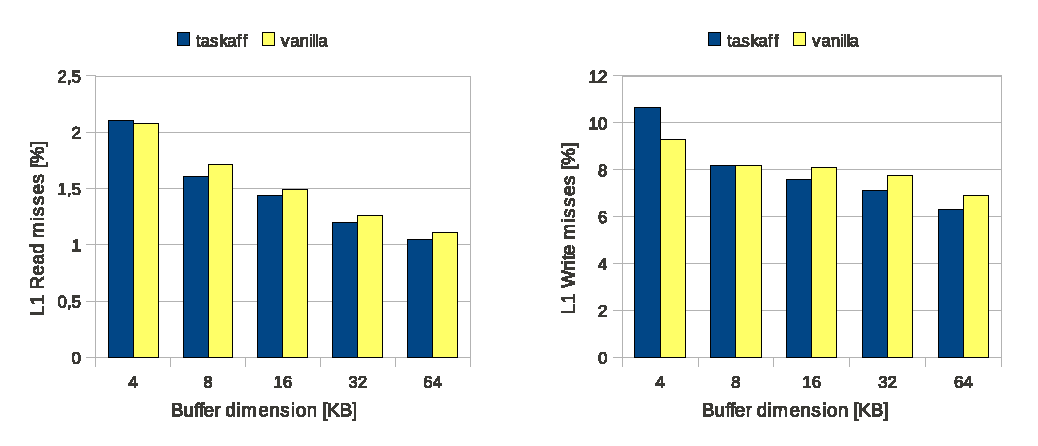
\includegraphics[width=\widefigure]{images/results_i7/l1_load_store_i7.eps}
\caption{\figurecaption{L1 Read and Write misses on Xeon}}
\label{fig:l1_load_store_i7}
\end{figure}

\begin{figure}[htbp]
\centering
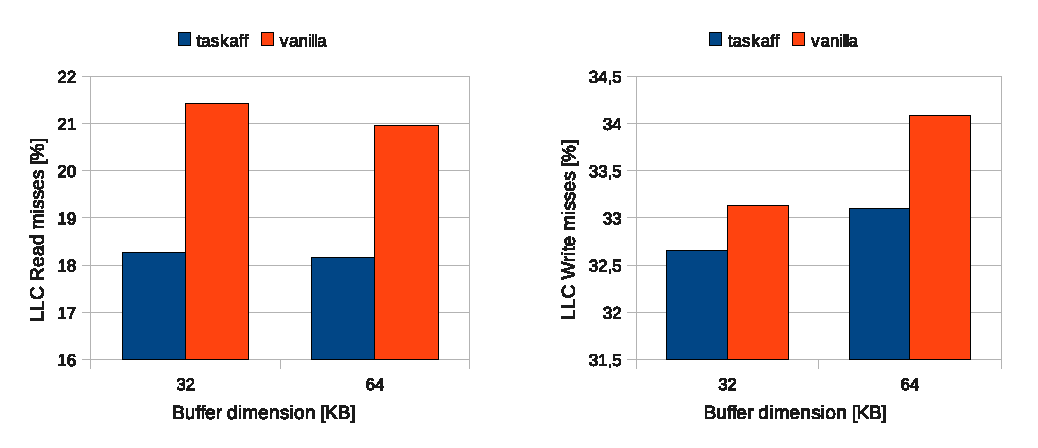
\includegraphics[width=\widefigure]{images/results_i7/l3_load_store_i7.eps}
\caption{\figurecaption{LLC Read and Write misses on Xeon}}
\label{fig:l2_load_store_i7}
\end{figure}

Also in this case expected scheduling is performed, Fig TODO, therefore there is a significant throughput improvement. As in the previous case, migration 
are greatly increased, but now both L1 and LLC miss rate are diminished, see Fig TODO. It is clear that architecture of i7 is better exploited by task 
affinity.  

On Intel i7, when a core requires a data, it sends a data request to L3 cache. If data is in L3 and there is a hit, the L3 cache query the "core valid" 
bits of the cache line that contains requested data, in order to know which is the core that owns requested data. The core that owns requested data reply to 
the request with the most recent copy of data. Instead on Intel Xeon, when core requires a data, only core in the same die can reply to the request, for 
example: if core A and core B are on the same chip and core A requires a data contained in L1 cache of the core C, the request of the core A results in a 
cache miss and data are retrieved from main memory. For this reason, L1 read and write miss rates on Intel i7 are lower than miss rates on Intel Xeon.

The same is true for LLC read and write miss rate, on Intel Xeon cores can retrieve data only from LLC cache of the same die, for this reason miss rates 
are higher than LLC miss rates.

TODO riassumendo tabella speedup


%%%%%%%%%%%%%%%%%%%%%%%%%%%%%%%%%%%%%%%%%%%%%%%%%%%%%%%%%%%%%%%%%%%%%%%%%%%%%
\section{AMD}

TODO solo il trace dicendo che non funziona



